\documentclass[11pt]{beamer}
\usepackage{listings} % Include the listings-package
\usepackage[T1]{fontenc}
\usepackage[utf8]{inputenc}
\usepackage[english]{babel}
\usepackage{amsmath}
\usepackage{amssymb, amsfonts, latexsym, cancel}
\usepackage{float}
\usepackage{graphicx}
\usepackage{epstopdf}
\usepackage{subfigure}
\usepackage{hyperref}
%\usepackage{authblk}
\usepackage{blindtext}
\usepackage{booktabs} % Allows the use of \toprule, 
\usepackage{filecontents}
\usepackage{courier} %% Sets font for listing as Courier.
\usepackage{listings}
%\usepackage{listings, xcolor}
\lstset{
tabsize = 2, %% set tab space width
showstringspaces = false, %% prevent space marking in strings, string is defined as the text that is generally printed directly to the console
numbers = left, %% display line numbers on the left
commentstyle = \color{green}, %% set comment color
keywordstyle = \color{blue}, %% set keyword color
stringstyle = \color{red}, %% set string color
rulecolor = \color{black}, %% set frame color to avoid being affected by text color
basicstyle = \small \ttfamily , %% set listing font and size
breaklines = true, %% enable line breaking
numberstyle = \tiny,
}
\usepackage{caption}
\DeclareCaptionFont{white}{\color{white}}
\DeclareCaptionFormat{listing}{\colorbox{gray}{\parbox{\textwidth}{#1#2#3}}}
\captionsetup[lstlisting]{format=listing,labelfont=white,textfont=white}
\definecolor{urlColor}{rgb}{0.06, 0.3, 0.57}
\definecolor{linkColor}{rgb}{0.57, 0.0, 0.04}
\definecolor{fileColor}{rgb}{0.0, 0.26, 0.26}
\hypersetup{
    colorlinks=true,
    linkcolor=linkColor,
    filecolor=fileColor,      
    urlcolor=urlColor,
}
\urlstyle{same}
\setbeamercovered{transparent}
%\usetheme{Boadilla}
\usetheme{CambridgeUS}
%\usetheme{Berkeley}
%\usetheme{Warsaw}
%\usetheme{Madrid}

\title[Inheritance]{\bf\Huge Inheritance}
\subtitle{Fundamentals to programming I}

\author[Plantilla De: rescobedoq]
{
	Glenny Shínderly Choque Vilcape\\
	Edisson Franklin Checalla Soto
}
\institute[UNSA]
{
\inst{1}% 
System Engineering School\\
System Engineering and Informatic Department\\
Production and Services Faculty\\
San Agustin National University of Arequipa
}

\date[2020-08-04]{\scriptsize{2020-08-04}}
%\logo{
\includegraphics[width=3.0cm]{img/logo_unsa.jpg}}
\titlegraphic{
\includegraphics[width=3.0cm]{img/logo_unsa.jpg}}

\begin{document}

\begin{frame}
\titlepage
\end{frame}

\begin{frame}
\frametitle{Content}
\tableofcontents
\end{frame}

\section{Introduction}
\begin{frame}
\frametitle{Introducction}
\begin{itemize}
\item The mechanism known as inheritance allows reusing classes: A new class is created that extends the functionality of an existing class without having to rewrite the code associated with it.
\end{itemize}
\end{frame}

\begin{frame}
\frametitle{Inheritance uml diagram}
the employee and constructor classes, in addition to the attributes and operations they define, inherit all their attributes and operations from the worker.
\begin{center}
{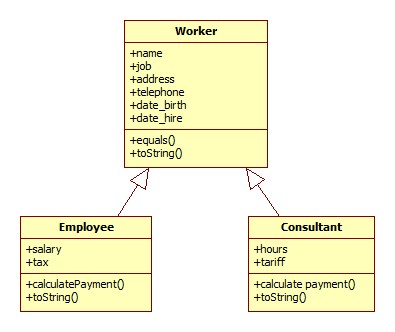
\includegraphics[width=7.0cm]{img/Herencia.jpg}}
\end{center}
\end{frame}

\begin{frame}
\frametitle{Employee uml diagram}
A particular employee will have, in addition to his or her attributes and operations as an employee, all the attributes corresponding to the worker superclass.

\begin{center}
{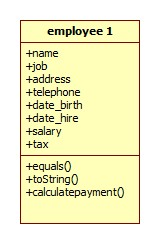
\includegraphics[width=4.0cm]{img/herencia2.jpg}}
\end{center}
\end{frame}


\begin{frame}
\section{Basic Example 1 }
%insertamos UML de Ejemplo 1 basico
\frametitle{UML Basic Example 1}
\begin{itemize}
\item \url{https://youtu.be/4gdhl-iRZZg}
\end {itemize}
\begin{center}
{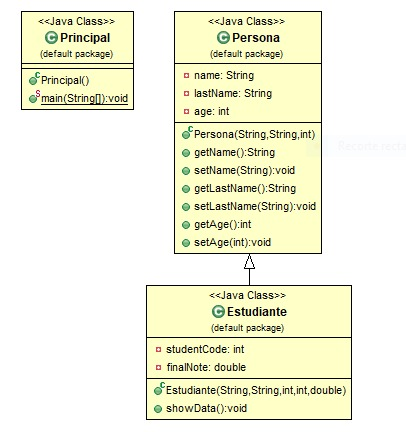
\includegraphics[width=6.0cm]{img/UmlBasicExample1.jpeg}}
\end{center}
\end{frame}

%Ejemplo Basico 1
\begin{frame}
\frametitle{Basic Examples 1- class Person (Part 1)}
\lstinputlisting[language=Java, firstline=1, lastline=16, label=hello-world, caption=Persona.java]{java/Basic Example 1/Persona.java}
\end{frame}
% ejemplo basico 1 clase persona
\begin{frame}
\frametitle{Basic Examples 1 - class Person (Part 2)}
\lstinputlisting[language=Java, firstline=17, label=hello-world, caption=Persona.java]{java/Basic Example 1/Persona.java}
\end{frame}
% ejemplo basico 1 clase estudiante
\begin{frame}
\frametitle{Basic Examples 1 - class Student}
\lstinputlisting[language=Java, label=hello-world, caption=Estudiante.java]{java/Basic Example 1/Estudiante.java}
\end{frame}
% ejemplo basico 1 clase principal
\begin{frame}
\frametitle{Basic Examples 1 - class Principal}
\lstinputlisting[language=Java, label=hello-world, caption=Principal.java]{java/Basic Example 1/Principal.java}
\end{frame}

%Ejemplo basico(Ejecución)
\begin{frame}
\frametitle{BAsic Example 1- Program Run}
\begin{center}
{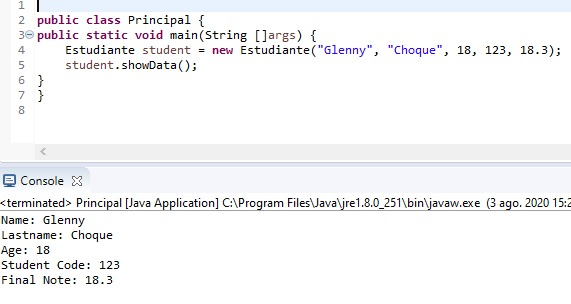
\includegraphics[width=12.0cm]{img/RunBasicExample1.png}}
\end{center}
\end{frame}


%sobrecarga de metodos
\begin{frame}
\section{Method override}
%insertamos UML de Ejemplo 1 basico
\frametitle{Method override}
\begin{itemize}
\item A subclass inherits all the methods of its superclass that are accessible to that subclass unless the subclass overwrites the methods.

\item A subclass overwrites a method of its superclass when it defines a method with the same characteristics (name, number, and type of arguments) as the method of the superclass.

\item Subclasses use method overwriting most of the time to add or modify the functionality of the parent class's inherited method.
\end{itemize}
\end{frame}

\begin{frame}
\section{Basic Example 2}
\frametitle{Basic Example 2 - UML Diagram Representation}
\begin{center}
{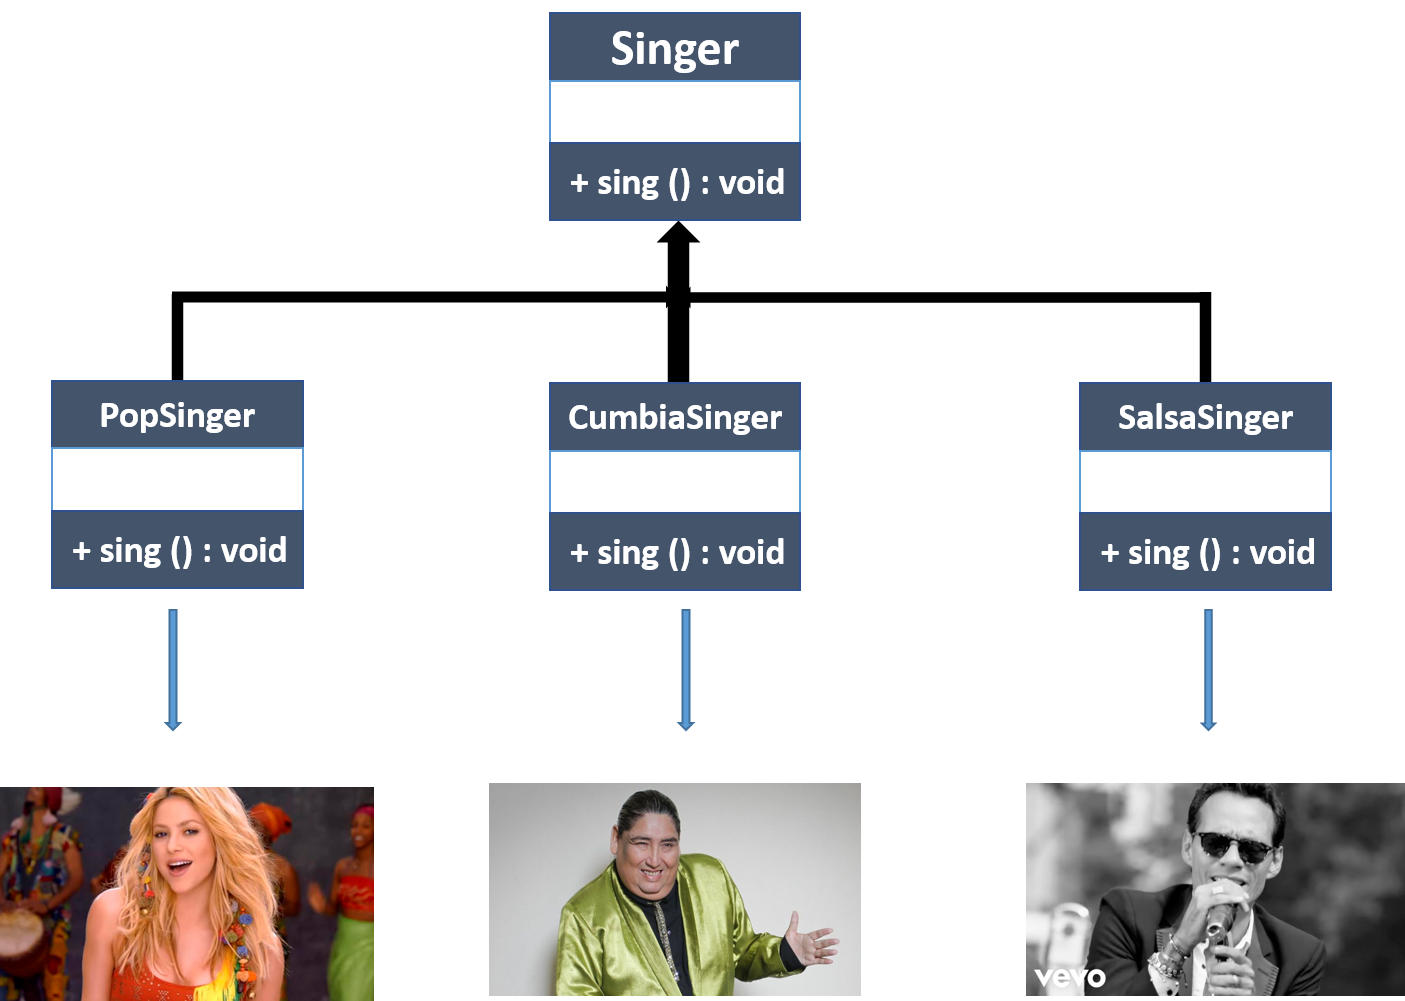
\includegraphics[width=10.0cm]{img/UmlSobreEscritura.png}}
\end{center}
\end{frame}

%Ejemplo Basico 2(Sobreescritura de metodos - Singer.java)
\begin{frame}
\frametitle{Basic Examples 2- class Singer}
\lstinputlisting[language=Java, firstline=1, lastline=16, label=hello-world, caption=Singer.java]{java/Basic Example 2/Singer.java}
\end{frame}

%Ejemplo Basico 2(Sobreescritura de metodos - PopSinger.java)
\begin{frame}
\frametitle{Basic Examples 2- class PopSinger}
\lstinputlisting[language=Java, firstline=1, lastline=16, label=hello-world, caption=PopSinger.java]{java/Basic Example 2/PopSinger.java}
\end{frame}

%Ejemplo Basico 2(Sobreescritura de metodos - SalsaSinger.java)
\begin{frame}
\frametitle{Basic Examples 2- class SalsaSinger}
\lstinputlisting[language=Java, firstline=1, lastline=16, label=hello-world, caption=SalsaSinger.java]{java/Basic Example 2/SalsaSinger.java}
\end{frame}

%Ejemplo Basico 2(Sobreescritura de metodos - CumbiaSinger.java)
\begin{frame}
\frametitle{Basic Examples 2- class CumbiaSinger}
\lstinputlisting[language=Java, firstline=1, lastline=16, label=hello-world, caption=CumbiaSinger.java]{java/Basic Example 2/CumbiaSinger.java}
\end{frame}

%Ejemplo Basico 2(Sobreescritura de metodos - Main.java)
\begin{frame}
\frametitle{Basic Examples 2- class CumbiaSinger}
\lstinputlisting[language=Java, firstline=1, lastline=16, label=hello-world, caption=Main.java]{java/Basic Example 2/Main.java}
\end{frame}

\begin{frame}
\frametitle{Basic Example 2 - Program Rum}
\begin{center}
{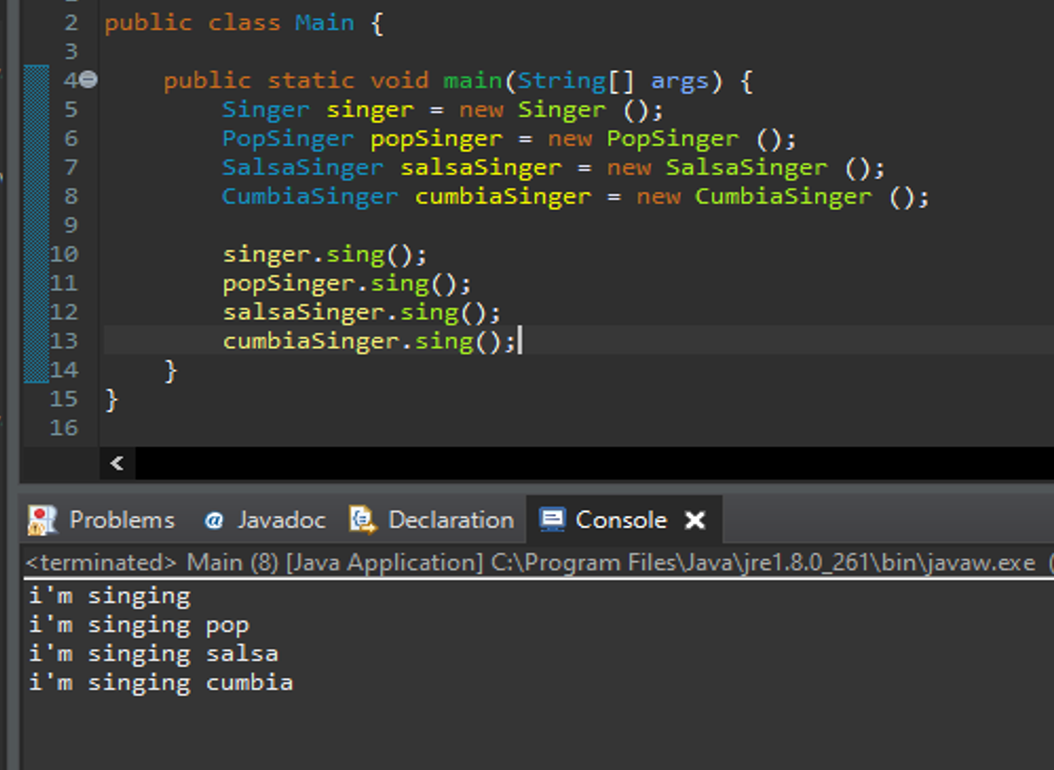
\includegraphics[width=10.0cm]{img/RunBasic1.png}}
\end{center}
\end{frame}



\begin{frame}
\section{Advanced Example 1}
\frametitle{Advanced Example 1 - UML Diagram Representation}
\begin{itemize}
\item \url{https://youtu.be/sGNhcWFLOJ8}
\end{itemize}
\begin{center}
{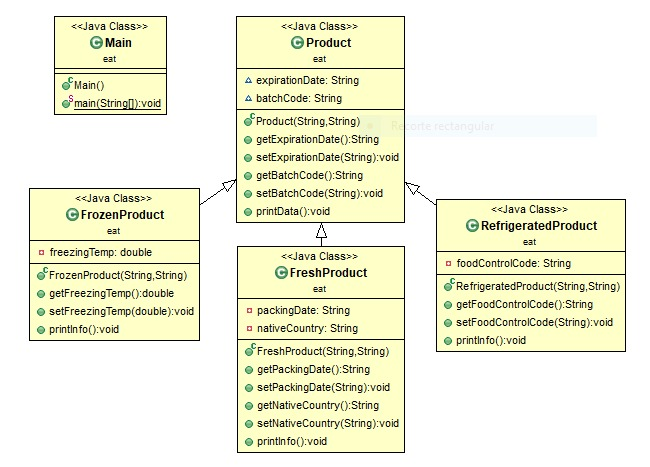
\includegraphics[width=10.0cm]{img/UmlAdvanced1.jpeg}}
\end{center}
\end{frame}

%Ejemplo avanzado1(producto.java)
\begin{frame}
\frametitle{Advance Example 1- class product (Part 1)}
\lstinputlisting[language=Java, firstline=1, lastline=12, label=hello-world, caption=Product.java]{java/Advanced Example 1/Product.java}
\end{frame}

\begin{frame}
\frametitle{Advance Example 1- class product (Part 2)}
\lstinputlisting[language=Java, firstline=13,  label=hello-world, caption=Product.java]{java/Advanced Example 1/Product.java}
\end{frame}

%Ejemplo avanzado1(FrozenProduct.java)
\begin{frame}
\frametitle{Advance Example 1- class FrozenProduct}
\lstinputlisting[language=Java, firstline=1, label=hello-world, caption=FrozenProduct.java]{java/Advanced Example 1/FrozenProduct.java}
\end{frame}

%Ejemplo avanzado1(FreshProduct.java parte 1)
\begin{frame}
\frametitle{Advance Example 1- class FreshProduct (Part 1)}
\lstinputlisting[language=Java, firstline=1,lastline=12, label=hello-world, caption=FreshProduct.java]{java/Advanced Example 1/FreshProduct.java}
\end{frame}

%Ejemplo avanzado1(FreshProduct.java parte 2)
\begin{frame}
\frametitle{Advance Example 1- class FreshProduct (Part 2)}
\lstinputlisting[language=Java, firstline=13, label=hello-world, caption=FreshProduct.java]{java/Advanced Example 1/FreshProduct.java}
\end{frame}

%Ejemplo avanzado1(RefrigeratedProduct.java)
\begin{frame}
\frametitle{Advance Example 1- class RefrigeratedProduct}
\lstinputlisting[language=Java, label=hello-world, caption=RefrigeratedProduct.java]{java/Advanced Example 1/RefrigeratedProduct.java}
\end{frame}

%Ejemplo avanzado1(RefrigeratedProduct.java)
\begin{frame}
\frametitle{Advance Example 1- class Main (Part 1)}
\lstinputlisting[language=Java,firstline =2,lastline =12 label=hello-world, caption=Main.java]{java/Advanced Example 1/Main.java}
\end{frame}

%Ejemplo avanzado1(RefrigeratedProduct.java)
\begin{frame}
\frametitle{Advance Example 1- class Main (Part 2)}
\lstinputlisting[language=Java,firstline =13, label=hello-world, caption=Main.java]{java/Advanced Example 1/Main.java}
\end{frame}

%Ejemplo avanzado 1(Ejecución)
\begin{frame}
\frametitle{Advance Example  1- Program Run}
\begin{center}
{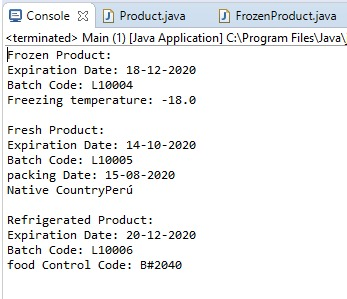
\includegraphics[width=8.0cm]{img/RunAdvanceExample1.png}}
\end{center}
\end{frame}

\begin{frame}
\section{Advanced Example 2}
\frametitle{Advanced Example 2 -statement}
Make a program to calculate the area of Polygons (Triangles and Rectangles) the program should be able to store in an N array triangles and rectangles, and at the end show the area and data of each one. To do this, you will have the following: 
\begin{itemize}
\item A super class called Polygon.
\item A sub class called Rectangle.
\item A sub class called Triangle.
\end{itemize}
\end{frame}
%uml de ejercicio avanzado 2
\begin{frame}
\frametitle{Advanced Example 2 - UML Diagram Representation}
\begin{center}
{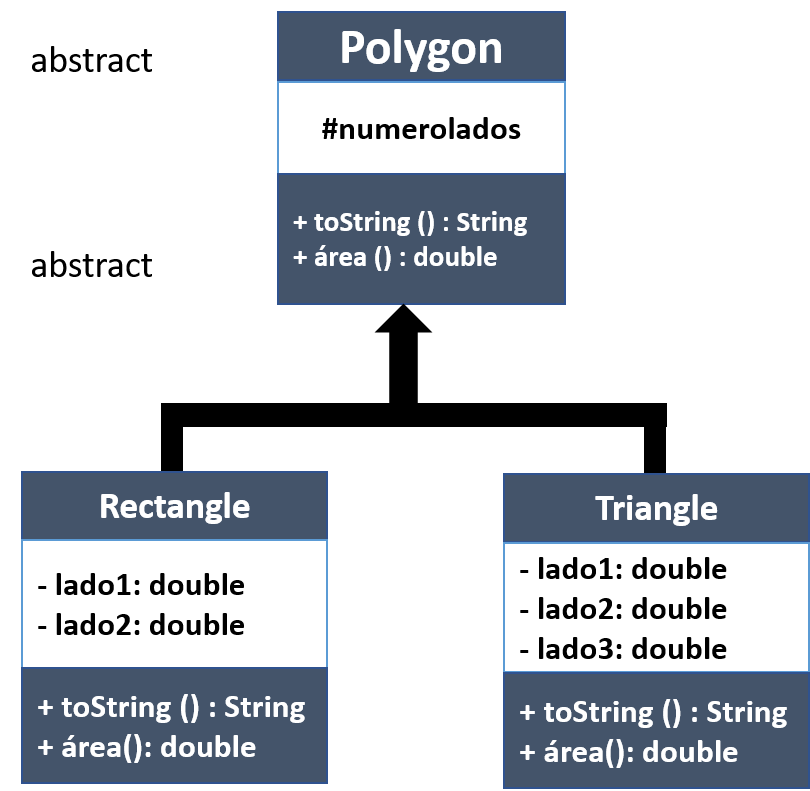
\includegraphics[width=7.5cm]{img/UmlAdvanceExample2.png}}
\end{center}
\end{frame}

%Ejemplo avanzado1(Polygon.java (Part 1))
\begin{frame}
\frametitle{Advance Example 2- class Polygon (Part 1)}
\lstinputlisting[language=Java,firstline = 1, lastline = 12, label=hello-world, caption=Polygon.java]{java/Advanced Example 2/Polygon.java}
\end{frame}

%Ejemplo avanzado1(Polygon.java (Part 2))
\begin{frame}
\frametitle{Advance Example 2- class Polygon (part 2)}
\lstinputlisting[language=Java,firstline = 13, label=hello-world, caption=Polygon.java]{java/Advanced Example 2/Polygon.java}
\end{frame}

%Ejemplo avanzado2(Rectangle.java (Part 1))
\begin{frame}
\frametitle{Advance Example 2- class Rectangle (Part 1)}
\lstinputlisting[language=Java,firstline = 1, lastline = 15 label=hello-world, caption=Rectangle.java]{java/Advanced Example 2/Rectangle.java}
\end{frame}

%Ejemplo avanzado2(Rectangle.java (Part 1))
\begin{frame}
\frametitle{Advance Example 2- class Rectangle (Part 2)}
\lstinputlisting[language=Java,firstline = 16, label=hello-world, caption=Rectangle.java]{java/Advanced Example 2/Rectangle.java}
\end{frame}

%Ejemplo avanzado2(Triangle.java (Part 1))
\begin{frame}
\frametitle{Advance Example 2- class Triangle(Part 1)}
\lstinputlisting[language=Java,firstline = 1, lastline=15 label=hello-world, caption=Triangle.java]{java/Advanced Example 2/Triangle.java}
\end{frame}
%Ejemplo avanzado2(Triangle.java (Part 2))
\begin{frame}
\frametitle{Advance Example 2- class Triangle(Part 2)}
\lstinputlisting[language=Java,firstline = 16, lastline=31 label=hello-world, caption=Triangle.java]{java/Advanced Example 2/Triangle.java}
\end{frame}

%Ejemplo avanzado2(Triangle.java (Part 3))
\begin{frame}
\frametitle{Advance Example 2- class Triangle(Part 3)}
\lstinputlisting[language=Java,firstline = 32,lastline = 41, label=hello-world, caption=Triangle.java]{java/Advanced Example 2/Triangle.java}
\end{frame}
%Ejemplo avanzado2(Triangle.java (Part 4))
\begin{frame}
\frametitle{Advance Example 2- class Triangle(Part 4)}
\lstinputlisting[language=Java,firstline = 42, label=hello-world, caption=Triangle.java]{java/Advanced Example 2/Triangle.java}
\end{frame}

%Ejemplo avanzado2(Main.java (Part 1))
\begin{frame}
\frametitle{Advance Example 2- class Main(Part 1)}
\lstinputlisting[language=Java,firstline = 1, lastline =8, label=hello-world, caption=Main.java]{java/Advanced Example 2/Main.java}
\end{frame}

%Ejemplo avanzado2(Main.java (Part 2))
\begin{frame}
\frametitle{Advance Example 2- class Main(Part 2)}
\lstinputlisting[language=Java,firstline = 9, lastline =15, label=hello-world, caption=Main.java]{java/Advanced Example 2/Main.java}
\end{frame}

%Ejemplo avanzado2(Main.java (Part 3))
\begin{frame}
\frametitle{Advance Example 2- class Main(Part 3)}
\lstinputlisting[language=Java,firstline = 16, lastline =27, label=hello-world, caption=Main.java]{java/Advanced Example 2/Main.java}
\end{frame}


%Ejemplo avanzado2(Main.java (Part 4))
\begin{frame}
\frametitle{Advance Example 2- class Main(Part 4)}
\lstinputlisting[language=Java,firstline = 28, lastline =37, label=hello-world, caption=Main.java]{java/Advanced Example 2/Main.java}
\end{frame}

%Ejemplo avanzado2(Main.java (Part 5))
\begin{frame}
\frametitle{Advance Example 2- class Main(Part 5)}
\lstinputlisting[language=Java,firstline = 38,lastline =48, label=hello-world, caption=Main.java]{java/Advanced Example 2/Main.java}
\end{frame}

%Ejemplo avanzado2(Main.java (Part 6))
\begin{frame}
\frametitle{Advance Example 2- class Main(Part 6)}
\lstinputlisting[language=Java,firstline = 49,lastline =59, label=hello-world, caption=Main.java]{java/Advanced Example 2/Main.java}
\end{frame}

%Ejemplo avanzado2(Main.java (Part 7))
\begin{frame}
\frametitle{Advance Example 2- class Main(Part 7)}
\lstinputlisting[language=Java,firstline = 60,lastline =70, label=hello-world, caption=Main.java]{java/Advanced Example 2/Main.java}
\end{frame}

%Ejemplo avanzado2(Main.java (Part 8))
\begin{frame}
\frametitle{Advance Example 2- class Main(Part 7)}
\lstinputlisting[language=Java,firstline = 71,label=hello-world, caption=Main.java]{java/Advanced Example 2/Main.java}
\end{frame}

%Ejemplo avanzado 2(Ejecución)
\begin{frame}
\frametitle{Advance Example  2- Program Run}
\begin{center}
{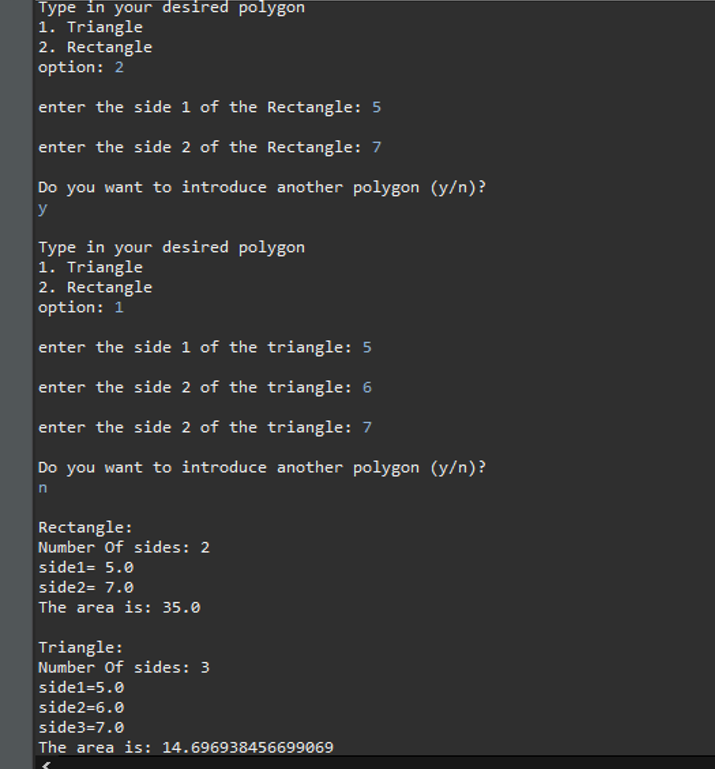
\includegraphics[width=7.0cm]{img/RunAdvancedExample2.png}}
\end{center}
\end{frame}

\section{References}
%References frame
\begin{frame}
\frametitle{References - Web pages}
\begin{itemize}
\item \url{https://elvex.ugr.es/decsai/java/pdf/9B-herencia.pdf}
\item \url{https://elvex.ugr.es/decsai/java/}
\item \url{https://aprenderaprogramar.com/foros/index.php?topic=2376.0}
\item \url{https://rua.ua.es/dspace/bitstream/10045/15995/1/POO-3-Herencia-10-11.pdf}

\end{itemize}
\end{frame}

\begin{frame}
\begin{center}
{
\includegraphics[width=8.0cm]{img/meme.jpeg}}
\end{center}
\begin{center}
Thanks!...
\
\end{center}
\end{frame}

\end{document}
